\documentclass[10pt,a4paper]{article}
\usepackage[margin=2.2cm]{geometry}
\usepackage{fontspec}
\usepackage{kotex}
\setmainfont{Apple SD Gothic Neo}
\setsansfont{Apple SD Gothic Neo}
\usepackage{amsmath,amssymb}
\usepackage{graphicx}
\usepackage{caption}
\usepackage[dvipsnames]{xcolor}
\usepackage[colorlinks=true,linkcolor=MidnightBlue,citecolor=MidnightBlue,
            urlcolor=MidnightBlue]{hyperref}
\usepackage{titlesec}
\titleformat{\section}{\large\bfseries}{\thesection}{0.6em}{}
\captionsetup{font=small,labelfont=bf}
\setlength{\parskip}{0.35em}
\setlength{\parindent}{0pt}
\usepackage{mdframed}
\newmdenv[linewidth=0.4pt,linecolor=gray!60,backgroundcolor=gray!5,
          innertopmargin=6pt,innerbottommargin=6pt,skipabove=8pt,skipbelow=8pt]{claimbox}
\newcommand{\claim}[2]{\begin{claimbox}\textbf{주장.} #1\par\smallskip
  \textcolor{gray!70}{\textbf{반증 조건.} #2}\end{claimbox}}

\title{\bfseries 합동은 배우지 않았다\\[2pt]
\large $\Delta(n)>0$ 창의 정체는 릿지의 어린 시절 --- 온보딩의 답은 적응이 아니라 라우팅}
\author{월드모델 실험실 · 노트 $851$ ($848$ 수확)}
\date{2026-08-09}
\begin{document}\maketitle

\section{한 줄}

챔피언 합동에 고객(KR 만화) 라벨을 $15{\sim}160$건 넣어 가며 로컬 릿지와
경주시켰다(격자 $5$ × 중첩 뽑기 $6$ × 씨앗 $12$ · $366$적합 · 체크포인트).
결과: \textbf{합동은 라벨로 적응하지 않는다} --- 끝점 기울기 $-0.0910$,
뽑기 $6$개 중 양수 $0$, $n \ge 80$ 에선 오히려 나빠진다($0.39 \to 0.30$).
$\Delta(n) > 0$ 인 창($n \le 40$ · $6/6$)은 합동의 실력이 아니라 \textbf{릿지가
아직 어린 구간}이고, 교차 $n^{\ddagger} \in (40, 80]$ 은 릿지의 학습곡선이
전이 상수 $\approx 0.39$ 를 넘는 지점일 뿐이다.

\begin{figure}[t]\centering
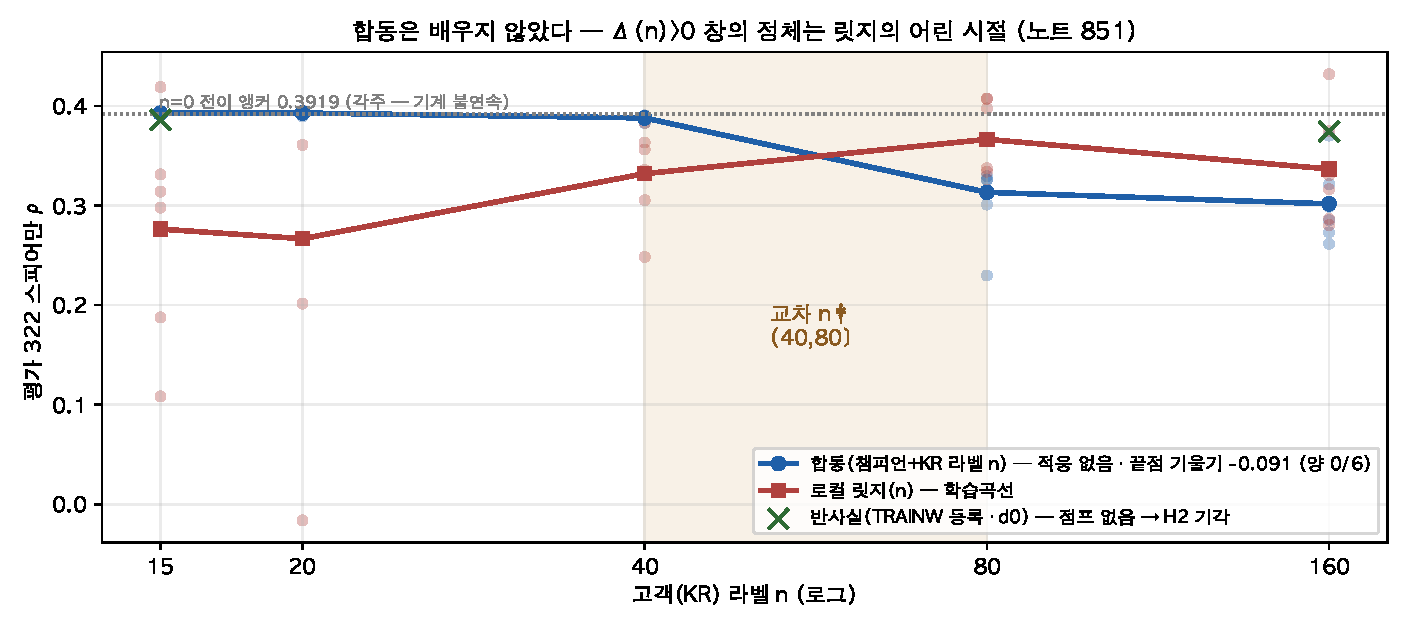
\includegraphics[width=0.97\textwidth]{figs/ridgeyouth.pdf}
\caption{합동(파랑)은 평평하다 못해 하강, 릿지(빨강)는 학습곡선. 초록 $\times$
= 반사실(TRAINW 등록) --- 점프 없음.}
\end{figure}

\claim{\textbf{T$1$ 파인튜닝 질문의 실측 답: 적응이 아니라 라우팅.}
판별 팔이 대안 기제를 죽였다 --- KR만화의 실효 도메인 가중은 클립 하한
$0.2$(산수 확정)인데, 가중을 정상 등록한 반사실 재적합($d0$ · $24$적합)에서도
$n{=}160$ 점프가 $+0.0041$ 뿐이다: \textbf{하한 교란(H$2$) 기각, `합동 기계는
새 도메인 라벨을 살리지 못한다'(H$1$) 확정.} 사업 문장 최종:
$843$(전이-단독 대 릿지)의 창은 $10{\sim}20$건, $851$(합동 대 릿지)의 창은
$40{\sim}80$건 --- 합동이 창을 $2{\sim}4$배 늘리지만 \textbf{그 이득은 전이
그 자체이지 라벨 학습이 아니다.} 고객 온보딩은 $n < n^{\ddagger}$ 전이 ·
$n > n^{\ddagger}$ 로컬 릿지로 갈아타는 라우팅이 정답이다.}
{joint 가 $n$ 이 커질수록 왜 나빠지는지는 모른다 --- H$1$ 은 관찰이지 기제가
아니다(기제 예측은 걸지 않는다: 반사실 점프에 $55\%$ 를 걸었다 또 틀렸고,
순서·문턱 예측은 $6$연속 적중대다). 반사실은 $d0$ 한정.}

\section{부속 --- 절단 정정과 다섯 번째 팔}

티처 \#$16$ 이 회사 필모 탭의 $10$편/페이지 절단을 적발했다(페이징은
\texttt{etcParam} --- \texttt{pageIndex} 는 조용히 무시). 전 페이지 재집계로
$850$ 의 `실적 $3/9$' 가 \textbf{$5/9$} 로 정정됐고(필름다빈 $0 \to 24$ ·
씨엠닉스 $0 \to 10$), `극장 통계 밖' 서사는 $4$개 회사로 축소됐다. 그 위에
annex$5$(v$3$ 채움 $5$편 · v$1$ 척도 유지)를 첫 라벨 관측 전에 봉인 ---
봉인 커버리지 사다리가 $56.7\% \to 83.3\%$ 에 닿았다. 수확($9/28$) 사다리:
$\rho_{v1} \cdot \rho_{격리(+3)} \cdot \rho_{v3(+5)} \cdot \rho_{v2(재척도)}$.
GitHub 흐름 $11$회째. 판 $\rho$ $0.4710$ 그대로.

\end{document}
